\chapter{Use Cases}
The Use Cases section defines specifics regarding the main, expected interactions between users and the system.
\begin{figure}
	\label{fig:useCase}
	\centering
	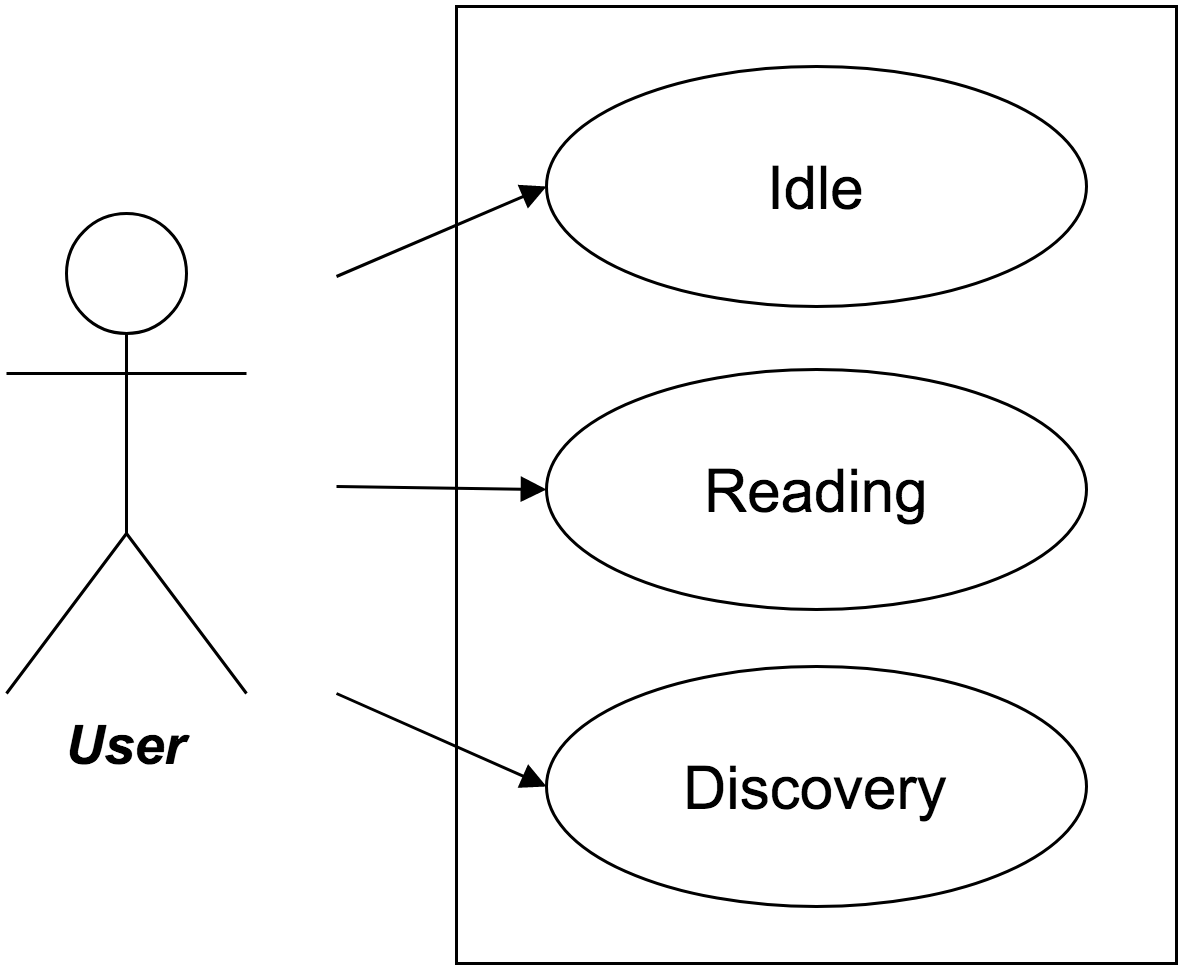
\includegraphics[scale = 0.4]{useCase.png}
    
    \caption{Use Cases}
\end{figure}

\pagebreak

\underline {"Gaze"}
\begin{description}
\item [Goal] Identify and obtain graphical input
\item [Actor] User
\item [Preconditions] Device must be turned on
\item [Steps] User stare at the document he will to know
\item [Postconditions] Graphical input pass to optical character recognition engine
\item [Exceptions] Unstable input, such that the motion of the headset is outside the threshold
\end{description}


\vspace{5mm}


\underline {Receive orientation feedback}
\begin{description}
\item [Goal] Inform the user to change the way he is looking at the document, such as tilt his head
\item [Actor] User
\item [Preconditions] Graphical input pass to optical character recognition engine
\item [Steps] Follow the instructions
\item [Postconditions] Graphical input pass to optical character recognition engine
\item [Exceptions] User choose not to recognize the text
\end{description}


\vspace{5mm}


\underline {Receive summary feedback}
\begin{description}
\item [Goal] Provides the user with a summary of the document
\item [Actor] User
\item [Preconditions] Document recognized by OCR and processed by text summarization engine
\item [Steps] Auto output to user after successful scan for document
\item [Postconditions] Request user for content feedback
\item [Exceptions] User choose to abort
\end{description}


\vspace{5mm}
\pagebreak

\underline {Receive content feedback}
\begin{description}
\item [Goal] Provides the user with the content of the document
\item [Actor] User
\item [Preconditions] User received summary feedback and wished more detailed content
\item [Steps] After the user listen to the summary feedback, he can press the control button to initiate the action
\item [Postconditions] N/A
\item [Exceptions] User choose to abort
\end{description}


